\documentclass[]{cv-etienne}

\usepackage[american]{babel}

\usepackage[autostyle]{csquotes}
%\usepackage{graphix}

\usepackage{fontawesome}

\addbibresource{curriculum.bib}

\hypersetup{%
  colorlinks=false,% hyperlinks will be black
  linkbordercolor=red,% hyperlink borders will be red
  pdfborderstyle={/S/U/W 1}% border style will be underline of width 1pt
}

\newfontfamily{\FA}{FontAwesome Regular}


\begin{document}
\header{Etienne}{Delay}{Researcher in social geography and  spatial modelling}

\begin{aside} % In the aside, each new line forces a line break
%\includegraphics[width=largeur]{nom du fichier}
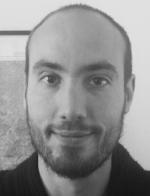
\includegraphics{img/delay_s}
\section{Personnel}
Age :  32 ans
Situation : PACS
\section{Contact}
UPR GREEN
Campus Baillarguet
34398 Montferriez-su-lez
~
+33 614 325 300
%+221 77 459 90 43
~
{\color{lightgray}{\FA \faEnvelope}} \href{mailto:etienne.delay@cirad.fr}{\footnotesize etienne.delay@cirad.fr}
{\color{linkedin}{\FA \faLinkedin}} \href{https://www.linkedin.com/in/etienne-delay-8871a45b/}{\footnotesize https://goo.gl/zKk9Yu}
{\color{twitter}{\FA \faTwitter}} {\footnotesize \href{https://twitter.com/ElCep}{@ElCep}}
{\color{github}{\FA \faGithub}} {\footnotesize \href{https://github.com/ElCep}{ElCep}}
{\color{lightgray}{\FA \faHome}} {\footnotesize \href{http://elcep.legtux.org}{http://lamenagerie.org}}
\section{Languages}
Français : native
English : academic
Italian : bilingual
\section{Programming}
{\color{red} $\varheartsuit$} R, Netlogo
SQL and dialects
\LaTeX, UML,
\section{Software}
{\color{red} $\varheartsuit$} Linux \& Unix-like,
Netlogo, {\color{red} $\varheartsuit$} OpenMole,
{\color{red} $\varheartsuit$} Gama-plateform,
QGIS, GRASS, Mapserver,
PostgreSQL, PostGIS,
pgRouting, MySQL
\end{aside}

\section{Profile}
To tackle the scientific challenges proposed by landscape dynamics and cooperation processes, I have developed a research methodology based on field work and companion modelling combined with the formalisation of the observed processes and agents based models.\\
This approach offers the possibility to understand : spatial, social, cultural and / or economic conditions that take place on territories, and to provide prospective scenarios. \\
These methods have been applied in various contexts: steep slope vineyards landscapes (2011), water resource management cooperation (2015), vegetation cover in dry climate (2017). The established research networks are still active through sustained collaborations and activities.

My technical expertise grew and evolved through investment in several workgroups: MAPS Team (Modelling Applied to Space Phenomena), OSGeo (president of the OSGeo's French chapter since 2013, member of the OSGeo-international chapter since 2015), various initiatives around modelling, exploration and sensibility analysis of spatial patterns behaviours, and more generally in Free Software communities.

I also enjoy travelling, zetetic and running.
\vspace{2em}

\section{Partnerships}
\begin{entrylist}
%------------------------------------------------
\entry
{Since 2017}
{ANR Future Sahel {\normalfont led by D. Goffner}}
{UMI 3189 CNRS,  SNG}
{\emph{The Future Sahel program} is financed by the French research agency. Its goal is to provide scientific help and support to the national agency for the great green wall in Senegal.}
%------------------------------------------------
\end{entrylist}

\begin{entrylist}
%------------------------------------------------
\entry
{2016}
{COMMONS program {\normalfont led by M. Chevallier and E. Delay}}
{UMR 6042 CNRS, FR}
{\emph{The COMMONS program} (\textit{COllective ManageMent Of Natural reSources}) is financed by the AOI funding of Limoges University, and aims to structure an international research network about cooperation in an interdisciplinary way. This network is focused on collective management of natural resources.}
%------------------------------------------------
\end{entrylist}
\begin{entrylist}
%------------------------------------------------
\entry
{Since 2015}
{LittoSim project {\normalfont led by N. Becu}}
{UMR 7266 CNRS, FR}
{\emph{The LittoSim project} is funded by the "Défi Littoral" action from CNRS. This project brings together 11 French researchers. Our goal : develop a pedagogical tool for raising developers and government awareness about risks of marine submersion.}
%------------------------------------------------
\end{entrylist}

\begin{entrylist}
%------------------------------------------------
\entry
{Since 2014}
{VitiTerroir program {\normalfont led by S. Leturcq and A. Lammoglia}}
{UMR 7324 CNRS, FR}
{\emph{VitiTerroir's purpose is to initiate a prospective tool based on modelling of terroirs' transformations within a long-term approach.}}
%------------------------------------------------
\end{entrylist}
\begin{entrylist}
%------------------------------------------------
\entry
{2012-2016}
{LACCAVE program {\normalfont led by N. Ollat and J-M. Touzard}}
{INRA, FR}
{\emph{Long-term impacts and Adaptation to Climate ChAnge in Viticulture and Enology.} This interdisciplinary program brings together 23 French research laboratories to assess the effects of climate change on the vine and wine, and to explore adaptation strategies amongst French wine regions. }
%------------------------------------------------
\end{entrylist}
\begin{entrylist}
%------------------------------------------------
\entry
{Since 2011}
{Ricerca sulla viticoltura di montagna  {\normalfont  led by M. Pontalti and F. Zottele \\}}
{ Fondazione E.MACH, Italiy}
{\emph{Studies and experimentation about sustaining a mountain viticulture in Trentino, and more widely about European issues}.
This work is conducted in partnership with the CERVIM (Center for studies and research on mountains and steep slope viticulture).}
%------------------------------------------------
\end{entrylist}
\begin{entrylist}
%------------------------------------------------
\entry
{2011-2016}
{ANR TerViClim {\normalfont led by H. Quénol}}
{ Rennes university, FR}
{\emph{Observation and spatial modelling of world wine regions climate in a context of climate change}:
Installation of temperature sensors throughout the AOC Banyuls-Collioure (Pyrénées Orientales, FR) and Val di Cembra (Trentino, IT).}
%------------------------------------------------
\end{entrylist}

\section{Scientific responsibilities}
\begin{entrylist}
%------------------------------------------------
\entry
{Jul. 2017}
{Scientific Committee Member for FOSS4G-eu}
{ENSG - Marne-la-Vallée - FR}
{\emph{Free and Open Source Software for Geospatial congress} (FOSS4G). 3 days congress, bringing together FOSS4G European communities of developers and users in order to share ideas for improving geodata, software and applications openness.}
%------------------------------------------------
\end{entrylist}
\begin{entrylist}
%------------------------------------------------
\entry
{June 2017}
{Co-organiser of MAPS-10 CNRS Summer school}
{Oléron - FR}
{A one-week summer school labelled by the French national research center (CNRS). 30 participants working and learning together on spatial modelling of socio-environmental phenomena.}
%------------------------------------------------
\end{entrylist}
\begin{entrylist}
%------------------------------------------------
\entry
{June 2017}
{Scientific Committee Member of the $20^{e}$ international GiESO congress}
{Mendoza (ARG)}
{Gathering 250 scientists and engineers from about 20 countries, the last advancements in Vitiviniculture are discussed at scientific and tech transfer level, with a focus on sustainable development.}
%------------------------------------------------
\end{entrylist}
\begin{entrylist}
%------------------------------------------------
\entry
{Nov. 2016}
{Scientific Committee Member for "Beyond institutional participation" workshop}
{Limoges university, FR}
{3-day workshop to produce an in-depth survey of governance and participatory approach in the water democracy.}
%------------------------------------------------
\end{entrylist}
\begin{entrylist}
%------------------------------------------------
\entry
{Since 2015}
{MAPS Team member}
{}
{MAPS is a French thematic network dealing with agent based models applied to spatialised phenomena. Every year, we organise interdisciplinary workshops to develop scientific simulations in the fields of complexity and agent based modelling}.
%------------------------------------------------
\end{entrylist}
\begin{entrylist}
%------------------------------------------------
\entry
{Since 2015}
{OpenMole Team member}
{ISC-PIF - Paris}
{OpenMOLE explores, diagnoses numerical model and optimizes its dynamics taking advantage of distributed computing environments. The typical usages are model calibration, model exploration, machine learning, optimization, data processing}.
%------------------------------------------------
\end{entrylist}
\begin{entrylist}
%------------------------------------------------
\entry
{June 2015}
{Scientific Committee Member for $19^{e}$ international GiESCO congress}
{Gruissan, FR}
{This congress is one of the main scientific and technological event in the field of Viticulture.}
%------------------------------------------------
\end{entrylist}
\begin{entrylist}
%------------------------------------------------
\entry
{2014-2016}
{Coordinator for FOSS4G-fr}
{ENSG - Marne-la-Vallée, FR}
{Free and Open Source Software for Geospatial congress (FOSS4G). The Conference aims to bring together FOSS4G francophone users and developers interactions with and amongst French and francophone communities in order to share ideas for improving geodata, software and applications openness.}
%------------------------------------------------
\end{entrylist}
\begin{entrylist}
%------------------------------------------------
\entry
{Nov. 2013}
{Co-organiser of the workshop "Agent based modelling and multi-model coupling."}
{SupAgro - Montpellier, FR}
{The aim of this interdisciplinary workshop is to build disciplinary agent based models and provide computing frameworks and tools to connect them. We have worked on vineyard and climate change context.}
%------------------------------------------------
\end{entrylist}
\begin{entrylist}
%------------------------------------------------
\entry
{June 2013}
{LACCAVE seminar organiser}
{Banyuls-sur-mer, FR}
{In this program, I organised a seminar about adaptation and climate change in viticulture through a professional and scientific transfer perspective, in order to enlighten professional expectation and scientific progress}
%------------------------------------------------
\end{entrylist}

\section{Education}

\begin{entrylist}
%------------------------------------------------
\entry
{2011-2015}
{PhD candidate in geography {\normalfont GEOLAB UMR 6042 CNRS}}
{Limoges university, FR}
{\emph{Evolution and landscape prospective on steep slope areas} Case studies : Banyuls-Collioure AOC (Eastern Pyrenees, France) and Val di Cembra (Trentino, Italy). \\Supervisors: Eric \textsc{Rouvellac}, Nicolas \textsc{Becu} and Philippe \textsc{Allée}.}
%------------------------------------------------
\end{entrylist}

\begin{entrylist}
%------------------------------------------------
\entry
{2009-2011}
{DEUST {\normalfont "Webmaster et gestionnaire d’intranet"}}
{Limoges university, FR}
{\emph{Web languages and networks management}}
%------------------------------------------------
\end{entrylist}

\begin{entrylist}
%------------------------------------------------
\entry
{2008-2011}
{L3, M1, M2 {\normalfont "Heritage and spatial planning valuation"}}
{ Limoges university, FR}
{\emph{Territorial development of rural areas.}}
%------------------------------------------------
\end{entrylist}

\begin{entrylist}
%------------------------------------------------
\entry
{2006-2008}
{BTSA {\normalfont Management Nature Conservation}}
{ CFPPA, la Côte-Saint-André, FR}
{\emph{Specialty : Management of natural wilderness}}
%------------------------------------------------
\end{entrylist}

\begin{entrylist}
%------------------------------------------------
\entry
{2004-2006}
{Biology L1 \& L2}
{Joseph \textsc{Fourier} University, Grenoble, FR}
{\emph{Speciality : modelling natural phenomena (R-project \& Berkley Madonna).}}
%------------------------------------------------
\end{entrylist}

\section{Experience}
\begin{entrylist}
%------------------------------------------------
\entry
{Since 2018}
{GREEN research unit}
{CIRAD - Montpellier (FR)}
{\emph{Young Researcher}\\
Companion modelling and method development helping stockholders and decision makers involved in the mediation process. A special interest in cooperation emergence and maintain study regarding environmental condition.}
%------------------------------------------------
\end{entrylist}
\begin{entrylist}
%------------------------------------------------
\entry
{2017-2018}
{OHMi Téssékéré - Great Green Wall in Senegal}
{CNRS - Dakar, SNG}
{\emph{Post-doctoral fellowship} with J.-L. \textsc{Peiry}.\\
Tools development helping decision makers in the mediation process for the great green wall project. 12 months.}
%------------------------------------------------
\end{entrylist}
\begin{entrylist}
%------------------------------------------------
\entry
{March 2016}
{Doctoral studies center}
{IBN ZOHR university, Agadir, Morocco}
{\emph{Lecturer} \\
 Joint organisation of an agent based modelling training week to PhD candidates in Agadir.}
%------------------------------------------------
\end{entrylist}
% \begin{entrylist}
% %------------------------------------------------
% \entry
% {Mars 2016}
% {Doctoral studies center}
% {IBN ZOHR university, Agadir, Morocco},
% {\emph{lecturer} \\
% Joint organisation an agent based modelling training week to the PhD candidate in Agadir.}
% \end{entrylist}
\begin{entrylist}
%------------------------------------------------
\entry
{2015-2017}
{Chaire d'excellence Capital environnemental et gestion durable des cours d’eau}
{Limoges university, FR}
{\emph{Post-doctoral fellowship} with J. \textsc{Linton}. \\
Development of a social index of water quality. Generate statistically valid populations of artificial agents in order to test the social index. 16 months
}
\end{entrylist}

\begin{entrylist}
%------------------------------------------------
\entry
{2015}
{Research support}
{Limoges university, FR}
{\emph{Engineer} \\
IT infrastructure's implementation of a web-GIS (Geographic Information System) based on Debian, Mapserver, MySQL, Openlayer3 and Leaflet.
}
\end{entrylist}

\begin{entrylist}
%------------------------------------------------
\entry
{Since 2013}
{Department of Geography}
{Limoges university, FR}
{\emph{Lecturer} \\
A variety of Geography courses (100h), from L1 to M2, including statistic, cartography, social network analysis, geopolitic. Group lessons and student support with an e-learning platform (Moodle 2.X).
}
\end{entrylist}
%------------------------------------------------
\begin{entrylist}
\entry
{2011}
{Fondazion E. Mach}
{San Michele all Adige, IT}
{\emph{Engineer}\\
Project manager, from preliminary design studies to the setting up of map servers prototype's infrastructure. Work on LIDAR data for the detection of steep slope vineyards in Trentino (Italy)
}
\end{entrylist}
%------------------------------------------------
\begin{entrylist}
\entry
{2010}
{CERVIM}
{Aosta, IT}
{\emph{Internship}\\
Introduction of remote sensing inventory methods based on open source softwares (Qgis, GRASS, R). Setup of a collaborative work platform (Drupal and OpenAtrium).
}
\end{entrylist}
%------------------------------------------------
\begin{entrylist}
\entry
{2009}
{Alpine Ampelographic Center}
{Cevin, FR}
{\emph{Traineeship}\\
Implementation of inventory methods based on Geographic Information System (GIS), management of the documentation center.
}
\end{entrylist}
%------------------------------------------------
%\pagebreak
\section{Publications}
%\printbibsection{article}{Article in peer-reviewed journals}
\begin{refsection}
  \nocite{*}
  \printbibliography[type=article,title={Article in peer-reviewed journals},heading=subbibliography,sorting=ynt]
  \nocite{*}
  \printbibliography[type=incollection,title={Book chapters},heading=subbibliography,sorting=ynt]
  \nocite{*}
  \printbibliography[type=inproceedings,title={Peer-reviewed conferences},heading=subbibliography,sorting=ynt]
\end{refsection}

% \section{Price and Awards}
% %------------------------------------------------
% \begin{entrylist}
% \entry
% {2015}
% {Selected for the Jean-Claude Cassaing price}
% {Limoges university, Limoges, FR}
% {Reward the scientific aspects of Phd work and the doctor's ability to communicate his scientific work to the scientific community, and non-specialist public}
% \end{entrylist}
% %------------------------------------------------
% \begin{entrylist}
% \entry
% {2015}
% {Best scientific poster}
% {Internationnal GiESCO congress, Gruissan, FR}
% {Awarded for best scientific poster with \enquote{ A virtual pest to test a real method of integrated pest management: agent-based models as a tool to explore the behavior of \textit{L. botrana} during mating disruption.}}
% \end{entrylist}


\end{document}
